\section{Thiết kế mạch trên Altium Design}

\subsection{Schematic}

\subsubsection{Design a 3.3V regulator}

Mạch chỉnh lưu 3.3V regulator sử dụng IC TPS5430DDA làm bộ chuyển đổi DC-DC giảm áp (step-down converter) với
khả năng hoạt động ở dải điện áp đầu vào rộng từ 5.5V đến 36V xuống ổn định ở 3.3 V để cung cấp nguồn đầu vào cho bo vi điều khiển ESP32-WROM-32.

\begin{figure}[!htbp]
    \centering
    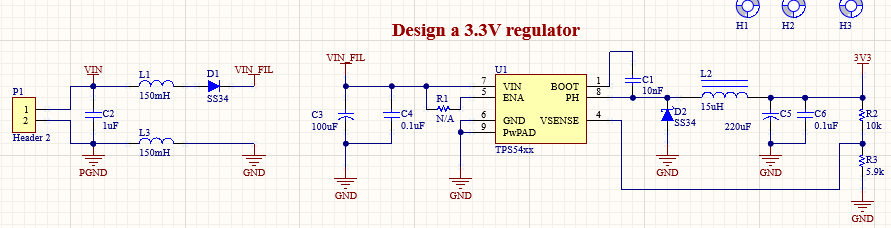
\includegraphics[width=\textwidth]{graphics/section3/f1.PNG}
\end{figure}

\subsubsection{Design a ESP32-WROM-32 part}
Bộ vi điều khiển ESP32-WROM-32 đóng vai trò là bộ xử lý chính trong mạch tổng hợp này.
\begin{figure}[!htbp]
    \centering
    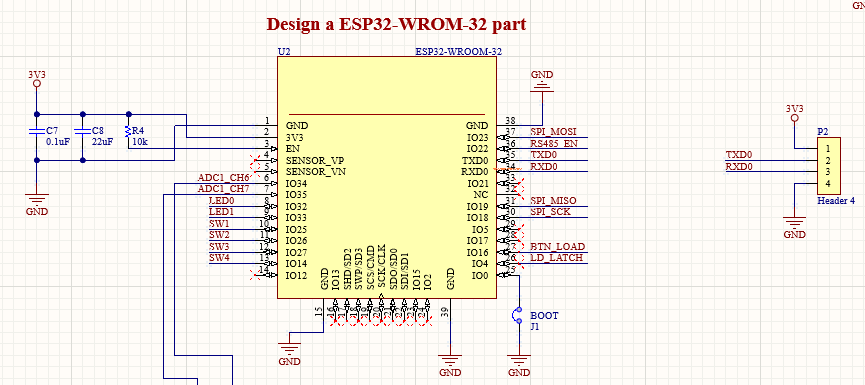
\includegraphics[width=\textwidth]{graphics/section3/f2.PNG}
\end{figure}

\subsubsection{Interfacing Slide Switch with an MCU}
\label{subsec: Interfacing Slide Switch with an MCU}

Công tắc SW DIP-4 điều khiển đầu vào cho các chân GPIO của bo vi điều khiển ESP32-WROM-32.

\begin{figure}[!htbp]
    \centering
    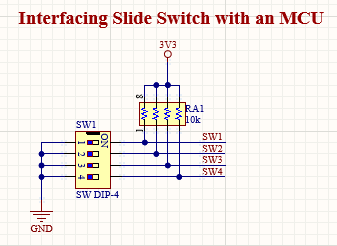
\includegraphics[width=0.3\textwidth]{graphics/section3/f3.PNG}
\end{figure}
\FloatBarrier

\subsubsection{Current sensor circuit}
\label{subsec:Current sensor circuit}

Mạch sử dụng bộ lọc thông thấp (low-pass filter) gồm điện trở, tụ điện và đệm tín hiệu qua opamp cho tín hiệu đo cảm biến dòng thông qua sử dụng 2 cảm biến dòng TA12 và TA17.
\begin{figure}[!htbp]
    \centering
    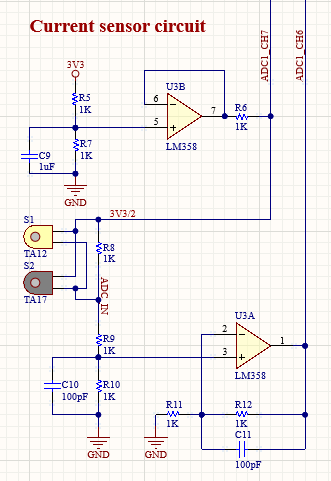
\includegraphics[width=0.3\textwidth]{graphics/section3/f4.PNG}
\end{figure}
\FloatBarrier

\subsubsection{Design a RS-485 part}
\label{subsec: Design a RS-485 part}
Mạch điều khiển giao tiếp RS-485 dùng IC MAX485 để chuyển đổi tín hiệu UART thành tín hiệu 485 và ngược lại và sử dụng RJ45x2 để kết nối tín hiệu RS-485.
\begin{figure}[!htbp]
    \centering
    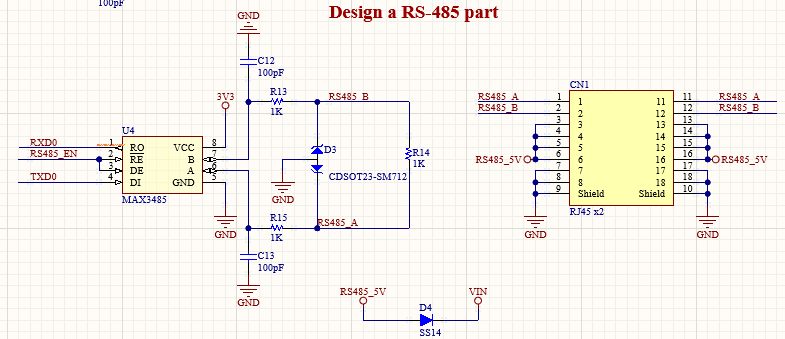
\includegraphics[width=\textwidth]{graphics/section3/f5.PNG}
\end{figure}
\FloatBarrier

\subsubsection{Interface with high-current LEDs}
\label{subsec: Interface with high-current LEDs}

Mạch điều khiển 2 LED đỏ và xanh thông qua tín hiệu từ 2 chân LED0 và LED1 của bộ vi điều khiển ESP32-WROM-32.
\begin{figure}[!htbp]
    \centering
    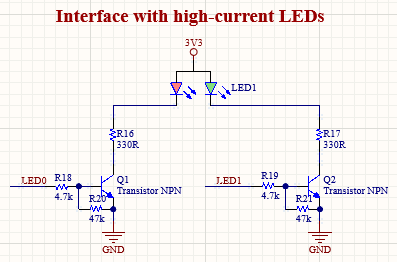
\includegraphics[width=0.7\textwidth]{graphics/section3/f6.PNG}
\end{figure}
\FloatBarrier

\subsection{PCB layout}
\begin{figure}[!htbp]
    \centering
    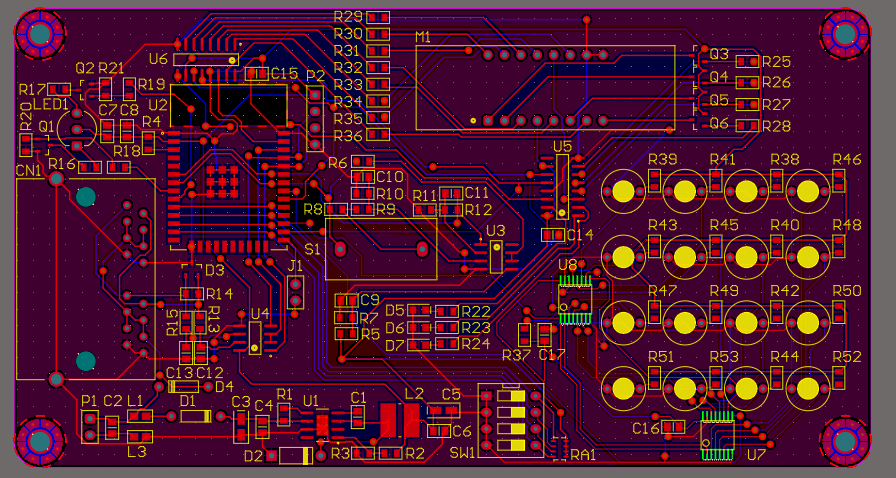
\includegraphics[width=\textwidth]{graphics/section3/f7.PNG}
    \caption{Top layer}
\end{figure}
\FloatBarrier

\begin{figure}[!htbp]
    \centering
    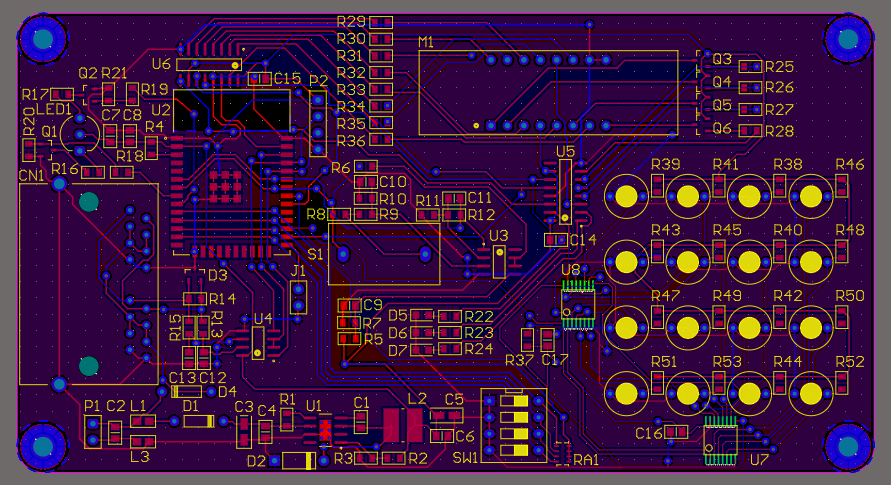
\includegraphics[width=\textwidth]{graphics/section3/f8.PNG}
    \caption{Bottom layer}
\end{figure}
\FloatBarrier
\subsection{Thành phẩm 3D}
\begin{figure}[!htbp]
    \centering
    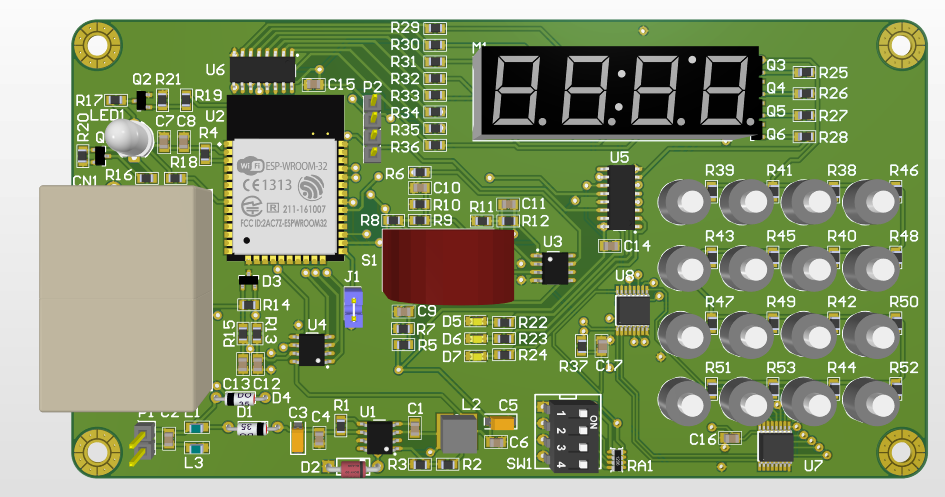
\includegraphics[width=\textwidth]{graphics/section3/f9.PNG}
    \caption{Top view}
\end{figure}
\FloatBarrier
\pagebreak
{ }
\begin{figure}[!htbp]
    \centering
    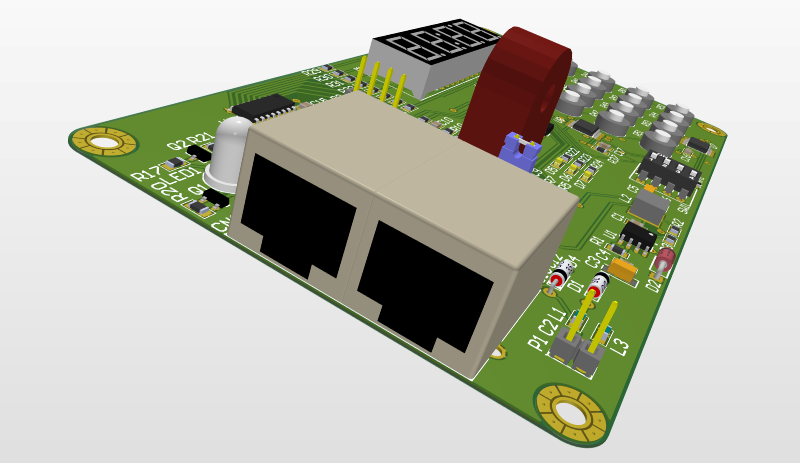
\includegraphics[width=\textwidth]{graphics/section3/f10.PNG}
    \caption{Isometric view}
\end{figure}
\FloatBarrier

